\documentclass[10pt,conference]{IEEEtran}

\makeatletter
\def\ps@headings{%
\def\@oddhead{\mbox{}\scriptsize\rightmark \hfil \thepage}%
\def\@evenhead{\scriptsize\thepage \hfil \leftmark\mbox{}}%
\def\@oddfoot{}%
\def\@evenfoot{}}
\makeatother
\pagestyle{headings}

% Load basic packages

\usepackage{amsmath}
\usepackage{balance}  % to better equalize the last page
\usepackage{graphicx}
\usepackage{subfigure}
\usepackage{graphics} % for EPS, load graphicx instead
\usepackage{times}    % comment if you want LaTeX's default font
\usepackage[hyphens]{url}      % llt: nicely formatted URLs
\usepackage{array}
\usepackage{enumerate}
\usepackage{algorithm2e}
\usepackage{color}
\usepackage{comment}
%\usepackage[bookmarks=false]{hyperref}


\newcommand{\todo}[1]{\textcolor{red}{TODO: #1}\\}

% llt: Define a global style for URLs, rather that the default one
%  \makeatletter
%  \def\url@leostyle{%
%   \@ifundefined{selectfont}{\def\UrlFont{\sf}}{\def\UrlFont{\small\bf\ttfamily}}}
%  \makeatother
%  \urlstyle{leo}


% To make various LaTeX processors do the right thing with page size.
\def\pprw{8.5in}
\def\pprh{11in}
\special{papersize=\pprw,\pprh}
\setlength{\paperwidth}{\pprw}
\setlength{\paperheight}{\pprh}
\setlength{\pdfpagewidth}{\pprw}
\setlength{\pdfpageheight}{\pprh}

% Make sure hyperref comes last of your loaded packages,
% to give it a fighting chance of not being over-written,
% since its job is to redefine many LaTeX commands.

% \usepackage[pdftex]{hyperref}
% \hypersetup{
% pdftitle={SIGCHI Conference Proceedings Format},
% pdfauthor={LaTeX},
%   pdfkeywords={SIGCHI, proceedings, archival format},
%   bookmarksnumbered,
%   pdfstartview={FitH},
%   colorlinks,
%   citecolor=black,
%   filecolor=black,
%   linkcolor=black,
%   urlcolor=black,
%   breaklinks=true,
% }

% create a shortcut to typeset table headings
\newcommand\litem[1]{\item{\bfseries#1\space:\space}}
\newcommand\tabhead[1]{\small\textbf{#1}}
\newcommand{\squeezeup}{\vspace{-3mm}}
\renewcommand{\labelitemi}{$\bullet$}
\renewcommand{\labelitemii}{$\cdot$}
\renewcommand{\labelitemiii}{$\diamond$}
\renewcommand{\labelitemiv}{$\ast$}
%\newcommand{\todo}[1]{\textcolor{red}{TODO: #1}}

\begin{document}
\title{SSD : Supervised Sarcasm Detection in Twitter using Social Cues}
%: Semi-Supervised Recognition of Sarcastic Sentences
%in Twitter and Amazon (CoNLL '10)}

\author{\IEEEauthorblockN{Swadhin Pradhan, Jian He}
\IEEEauthorblockA{CS, The University of Texas at Austin}}
% \IEEEauthorblockA{\IEEEauthorrefmark{2}CSE Department, Indian Institute of Technology Kharagpur, India}
% \IEEEauthorblockA{\IEEEauthorrefmark{3}CS Department, SUNY Korea}}


\date{20 April 2015}

\maketitle

%\renewcommand{\baselinestretch}{0.9}

%\begin{abstract}
This project si about detecting sarcasm.
\end{abstract}

\section{Introduction}
\textbf{Motivation :} In recent years, social media sites such as Twitter have gained immense popularity and importance. These sites have
evolved into large platforms where users express their ideas and opinions freely. Companies leverage this unique
ecosystem to tap into public opinion on their products or services and to provide real-time customer assistance. With the high velocity and volume of social media data, companies rely on tools such as HootSuite\footnote{https://hootsuite.com/}, to analyze data and to provide customer service. These tools perform tasks such as content management, sentiment analysis, and extraction of relevant messages for the company's customer service representatives to respond to. However, these tools lack the sophistication to decipher more nuanced forms of language such as sarcasm or humor, in which the meaning of a message is not always obvious and explicit.\\

Our goal in this project is to tackle the difficult problem of sarcasm detection on Twitter. While sarcasm detection
is inherently challenging, the style and nature of content on Twitter further complicate the process. Compared to other,
more conventional sources such as news articles and novels, Twitter is (1) more informal in nature with an evolving vocabulary of slang words and abbreviations and (2) has a limit of $140 $characters per tweet which provides fewer word level
cues and adds more ambiguity. However, it also different side channels to get some information about the context of a particular tweet like different hashtags, mentions, profile information, general sentiment of the named entities in tweets etc. To put the problem in a perspective, a few examples of sarcastic tweets from our experimental datasets are given below:
\begin{enumerate}
 \item \textit{Oh wow broken up 4 days and you've moved on already, thanks, don't feel like shit at all. \#sarcasm}.\\
 \item \textit{No my roommate play out of tune Zeppelin songs right outside my door isnt annoying. Not at all \#sarcasm \#sigh}.\\
 \item \textit{Wow! @TWCable\_NYC Thanks for the option of high speed internet at \$5 a month or 6 months free to save \$$0.30$ depending on the plan. \#sarcasm}.\\
 \item \textit{Man, Robinson Cano could be the laziest MVP ever \#sarcasm \#bigtimesarcasm}.\\
 \item \textit{20 minutes of laundry at 1 am. Awesome \#sarcasm}.\\
 \item \textit{Love walking through your cloud of cigarette smoke. Why buy my own pack when I can just inhale yours \#sarcasm}.\\
 \item \textit{Is everyone as excited about the \#GOP and \#Democrat conventions as I am?!? \#sarcasm \#serioussarcasm \#deepyawningmawofsarcaam}.\\
\end{enumerate}

\textbf{Our Approach :} Current research on sarcasm detection on Twitter \cite{riloff13,davidov10,tomas14,gonzalez_acl} has primarily focused on obtaining information from the text of the tweets. These techniques treat sarcasm as a linguistic phenomenon, with limited emphasis on the socio-contextual aspects of sarcasm. However, sarcasm has been extensively studied in psychological and behavioral sciences and theories explaining when, why, and how sarcasm is expressed have been established. All these works point that sarcasm is bound with broader common knowledge (e.g., about news or celebrities), the context known only to the author or author's opinion.\\

Hence, to follow a systematic approach, we first use and extend different lexical and syntactic features used in \cite{riloff13,davidov10,tomas14,gonzalez_acl} to capture the literal form of sarcasm. We explicitly utilize the occurrence of punctuation, stop words, slang, and emoticons which are very closely related to sentiment representation of tweets. Although twitter users think independently when updating their statuses, certain level of similarities in lexical structures are expected. Secondly, compared with normal tweets, more complicated syntactic structures may appear in sarcastic tweets so that implicit meaning of them can be understood by others. Syntactic complexity is an indicator of how easily the information of a tweet can be understood. Conventionally, sarcastic tweets convey messages implicitly, which possibly complicates syntactic structures. Finally and most importantly, we get different socio-contextual information from the information follower, followee, retweets, mentions etc. which represent the social context of the user and the tweet. So, we combine these features to train a supervised learning algorithm to detect sarcasm. We have collected sarcastic tweets with corresponding socio-contextual information using \#sarcasm hashtag and also later consolidated the dataset upto 75,253 tweets consisting 38,112 sarcastic tweets by getting tweets from the publicly available tweet ids from the authors of {riloff13,davidov10,tomas14}. We used SVM and ensemble technique like Logitboost or bagging to get the best F1-score of 0.9746 using this feature set in the above dataset.\\ 

\noindent We make the following contributions in this project:
\begin{itemize}
 \item We have created a Twitter dataset of reasonable amount of tweets with relevant socio-contextual information.
 \item To the best of our knowledge, we have employed sophisticated syntactic and social features to capture the context to better detect sarcasm. This approach can help in building language independent sarcasm detector.
 \item We believe that some classes of sarcastic tweets actually aimed at entities (e.g. may be person or institution or event or show) and so we have extracted the sentiment to get good indication of sarcasm.\\
\end{itemize}

In Sec. \ref{sec:related}, we review related sarcasm detection research. In Sec. \ref{sec:problem}, we formally define sarcasm detection on Twitter. In Sec. \ref{sec:dataset}, we discuss dataset collection procedure in detail and then we discuss the nature of different sarcastic tweets. In Sec. \ref{sec:features} we discuss different feature set and in Sec. \ref{sec:methodology} we describe the methodology employed in sarcasm detection. Next, in Sec. \ref{sec:evaluation}, we present experimental setup and different evaluation results. Finally, in Sec. \ref{sec:future} and Sec. \ref{sec:conclusion}, we conclude with different possible future directions.




%\input{eeg_primer}
%\section{Methodology and Experiment Setup}
\label{sec:methodology}
In this section, we will discuss in detail about umderlying working priniciples of SSD and different evaluation setups.
\subsection{Classifier Description}
We have initally attempted to train the system with simple unigram (bag of words), bigram, and tigram language model trained with $70\%$ of the tweets and testing with randomly selected $30\%$ of the tweets. For this binary classification task, we habe used SVM \cite{libsvm} with linear kernel and different ensemble techniques of boosting and bagging. Since we have a wide variety of features, we experimented with various ensemble learning techniques and found that LogitBoost performed best
empirically for boosting and bagging with SVM performed best for bagging technique. We used the Weka implementation of LogitBoost \cite{Friedman98} and EnsembleSVM for bagging \cite{ensembleSVM} to train a classifier using various combinations of features. We have used Decision Stumps as a base classifier in LogicBoost and ran boosting for 100 iterations. Furthermore, 
we have used SVM as a base classifier in bagging and ran bagging for 100 iterations. Training time of ensemble techniques were around $20$ hours in 8GB quadcore 3.2GHZ Ubuntu machine compared to around $1$ hour in SVM.

\subsection{Experiment Setup}

Fig. \ref{fig:infrastructure} shows the infrastructure of the whole system, which is divided into four parts: crawling module, parsing module, feature extracting module and sarcasm classifying module.

In the crawling module, we have developed a distributed crawling platform to collect a large-scale dataset from Twitter. The open-source tool Tweepy\cite{tweepy} was run on multiple machines in parallel, and all data will be centrally managed by the master node.

Raw tweets collected by the crawling module will be fed into the parsing module. The tool ark-twitter-nlp\cite{tweetnlp} was used to do tokenizing and POS tagging. After obtaining POS tagged tweets, TweeboParser\cite{kong2014dependency} will further run syntactic parsing which will generate syntactic dependency tree for each tweet. Named entity recognition was done by the tool in developed by Ritter et al\cite{Ritter11}\cite{Ritter12}. We applied sentiment analysis by utilizing the online machine learning framework Datumbox\cite{datumbox}. Due to the rate limit of this framework, we also created multiple parallel machine nodes to speed up sentiment analysis.

Parsed tweets are the input of the feature extracting module. We developed three feature extractors to extract corresponding features. After obtaining all tweet features, we are able to run the sarcasm classifying module, in which we used three classifiers, SVM with linear kernel, logitboosting with decision stump and bagging with SVM. 

\begin{figure}[htpb]
\centering
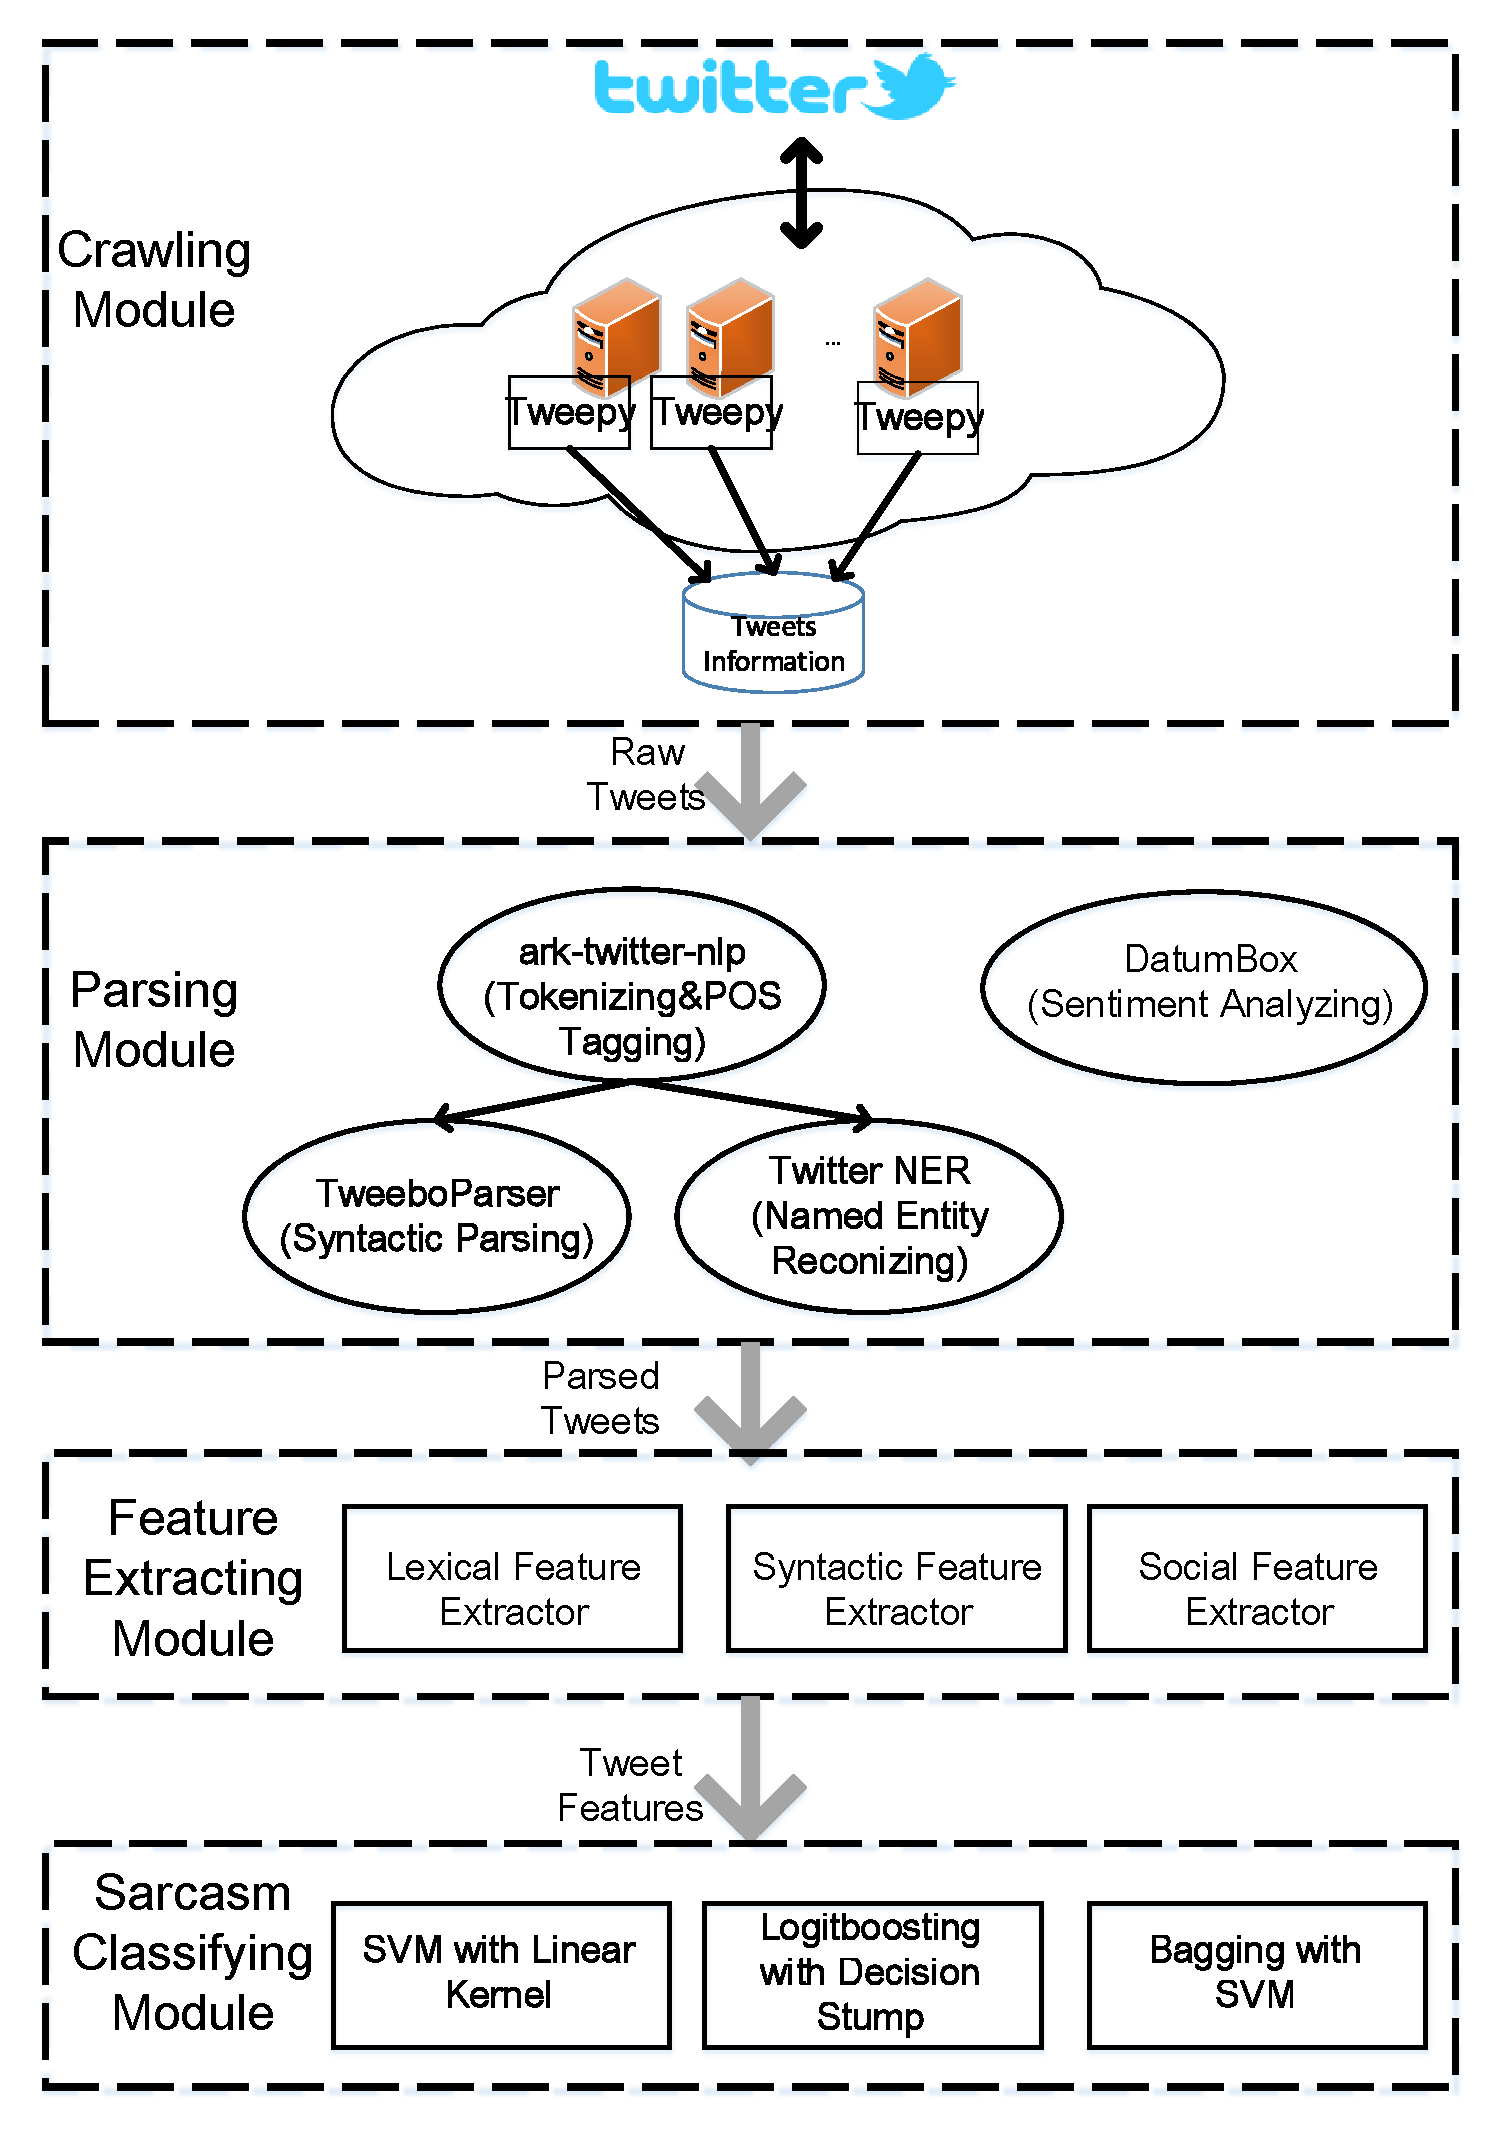
\includegraphics[scale=0.3]{infrastructure.eps}
\caption{The infrastructure of system setup.}
\label{fig:infrastructure}
\end{figure}

\section{Related Work}
\label{sec:related}
Sarcasm has been widely studied by psychologists, behavioral scientists and linguists for many years. Theories explaining the cognitive processes behind sarcasm usage such as the echoic reminder theory \cite{kreuz89}, allusional pretense theory \cite{kumon95}, and implicit display theory \cite{utsumi77} have been extensively researched. However, automatic detection of sarcasm is a relatively unexplored research topic and a challenging problem \cite{Pang2008}. While studies on automatic detection of sarcasm in speech \cite{tepper06} utilizes prosodic, spectral and contextual features, sarcasm detection in text has relied on identifying text patterns \cite{davidov10} and lexical features \cite{Kreuz07}.\\

Experiments with semi-supervised sarcasm identification on a Twitter dataset were conducted in \cite{davidov10}. They used 5-fold cross validation on their kNN-like classifier using mainly lexical features obtained an F-measure of 0.55 on the Twitter dataset. In \cite{davidov10}, authors use a semi-supervised sarcasm identification algorithm on a Twitter dataset and Amazon product reviews. In case of Twitter, authors mainly use $1500$ tweets containing \textit{\#sarcasm} hashtag and $180$ tweets tagged by $15$ Amazon Mechanical Turkers \cite{mturk} as golden test set or initial small labeled training set. The algorithm employs two modules: semi supervised pattern acquisition for identifying sarcastic patterns that serve as features for a classifier, and a classification stage that classifies each sentence to a sarcastic class. Reyes et al. \cite{reyes12} proposed features to capture properties of a figurative language such as ambiguity, polarity, unexpectedness and emotional scenarios. Their corpus consists of five categories (humor, irony, politics, technology and general), each containing 10,000 tweets. The best result in the classification of irony and general tweets was F-measure 0.65. Furthermore, Lukin and Walker \cite{Lukin_really13} explored the potential of a bootstrapping method for sarcasm classification in social dialogue to learn lexical N-gram cues associated with sarcasm (e.g., “oh really”, “I get it”, “no way”, etc.) as well as lexico-syntactic patterns. The work of Riloff et al. \cite{riloff13} identifies one type of sarcasm : contrast between a positive sentiment and negative situation. They used a bootstrapping algorithm to acquire lists of positive sentiment phrases and negative situation phrases from sarcastic tweets. Their evaluation on a human-annotated dataset of 3000 tweets (23\% sarcastic) was done using the SVM classifier with uni-grams and bigrams as features, achieving an F-measure of 0.48. \cite{gonzalez_acl} introduced a sarcasm detection technique using numerous lexical features (derived from LWIC \cite{pennebaker01} and Wordnet Affect \cite{valitutti04wordnet}) and pragmatic features such as emoticons and replies. Tomas et. al. \cite{tomas14} also tried to employ different combinations of machine learning approaches using language independent specific feature set on Czech and English Twitter dataset (780,000 tweets) and achieved F-measure around 0.94.
\section{Dataset Collection and Description}
\label{sec:dataset}
This is Dataset.
\section{Features}
\label{sec:features}
We will use three different groups of features to help improve sarcasm detection accuracy, including lexical features, syntactic features, and social features. Table \ref{tab:lexical features} shows the lexical features we used in our experiments. Lexical features mainly capture lexical patterns of tweets, such as common word usage, phrases, etc. Syntactic features illustrated in Table \ref{tab:syn features} represent syntactic structures of tweets, such as the simple SVO pattern, etc. We exploit social features listed in Table \ref{tab:social features} to characterize dependencies across tweets. For example, tweets with similar named entities tend to have same sentiments.

\begin{table}[htpb]
\centering
\begin{tabular}{|l|}
\hline
\tabincell{l}{Punctuation Frequencies\\
(The ratio between the number of punctuation \\
and the total number of tokens)} \\
\hline
Stopwords and Slang  \\
\hline
Emoticon Frequencies \\
\hline
Capitalization \\
\hline
Number of Hashtags and URLs \\
\hline
\tabincell{l}{Length of Sentence \\
(The number of tokens)}\\
\hline
Language Models(Unigram, Bigram and Trigram) \\              
\hline
\end{tabular}
\vspace{0.03 in}
\caption{Lexical Features}
\label{tab:lexical features}
\end{table}

\begin{table}
\centering
\begin{tabular}{|l|}
\hline
\tabincell{l}{Relative frequencies of different POS tags\\
parsed by the tool TweetNLP\cite{tweetnlp}\\
(The size of the tagset is $25$)}\\
\hline
\tabincell{l}{Fraction of words having syntactic function\\
(Syntactic dependency trees are generated by \\
TweeboParser\cite{kong2014dependency},some tokens do not \\
have syntactic function, such as ``RT'', ``@'', hashtags, etc.)} \\
\hline
\tabincell{l}{Number of inner nodes in dependency trees\\
(Phrases in a tweet can be characterized by subtrees,\\
thus the number of inner nodes is a reliable indicator\\
of the syntactic complexity of a tweet)}\\
\hline
\tabincell{l}{Sentiment of tweets\\
(The sentiment of a tweet can be positive,\\
negative or neutral. The online machine learning\\
framework Datumbox\cite{datumbox} is used to analyze sentiment.)}\\
\hline
\end{tabular}
\vspace{0.03 in}
\caption{Syntactic Features.}
\label{tab:syn features}
\end{table}

\begin{table}[htpb]
\centering
\begin{tabular}{|l|}
\hline
\tabincell{l}{Named Entities(The number of Named Entities,\\
the length of each named entity, the sentiment of each\\
named entity)}\\
\hline
\tabincell{l}{Social strength(The number of favorites,\\
the number of retweets, the follower count of the tweet\\
handler, the followee count of the tweet handler)}\\
\hline
\end{tabular}
\vspace{0.03 in}
\caption{Social Features}
\label{tab:social features}
\end{table}

\section{Methodology and Experiment Setup}
\label{sec:methodology}
In this section, we will discuss in detail about umderlying working priniciples of SSD and different evaluation setups.
\subsection{Classifier Description}
We have initally attempted to train the system with simple unigram (bag of words), bigram, and tigram language model trained with $70\%$ of the tweets and testing with randomly selected $30\%$ of the tweets. For this binary classification task, we habe used SVM \cite{libsvm} with linear kernel and different ensemble techniques of boosting and bagging. Since we have a wide variety of features, we experimented with various ensemble learning techniques and found that LogitBoost performed best
empirically for boosting and bagging with SVM performed best for bagging technique. We used the Weka implementation of LogitBoost \cite{Friedman98} and EnsembleSVM for bagging \cite{ensembleSVM} to train a classifier using various combinations of features. We have used Decision Stumps as a base classifier in LogicBoost and ran boosting for 100 iterations. Furthermore, 
we have used SVM as a base classifier in bagging and ran bagging for 100 iterations. Training time of ensemble techniques were around $20$ hours in 8GB quadcore 3.2GHZ Ubuntu machine compared to around $1$ hour in SVM.

\subsection{Experiment Setup}

Fig. \ref{fig:infrastructure} shows the infrastructure of the whole system, which is divided into four parts: crawling module, parsing module, feature extracting module and sarcasm classifying module.

In the crawling module, we have developed a distributed crawling platform to collect a large-scale dataset from Twitter. The open-source tool Tweepy\cite{tweepy} was run on multiple machines in parallel, and all data will be centrally managed by the master node.

Raw tweets collected by the crawling module will be fed into the parsing module. The tool ark-twitter-nlp\cite{tweetnlp} was used to do tokenizing and POS tagging. After obtaining POS tagged tweets, TweeboParser\cite{kong2014dependency} will further run syntactic parsing which will generate syntactic dependency tree for each tweet. Named entity recognition was done by the tool in developed by Ritter et al\cite{Ritter11}\cite{Ritter12}. We applied sentiment analysis by utilizing the online machine learning framework Datumbox\cite{datumbox}. Due to the rate limit of this framework, we also created multiple parallel machine nodes to speed up sentiment analysis.

Parsed tweets are the input of the feature extracting module. We developed three feature extractors to extract corresponding features. After obtaining all tweet features, we are able to run the sarcasm classifying module, in which we used three classifiers, SVM with linear kernel, logitboosting with decision stump and bagging with SVM. 

\begin{figure}[htpb]
\centering
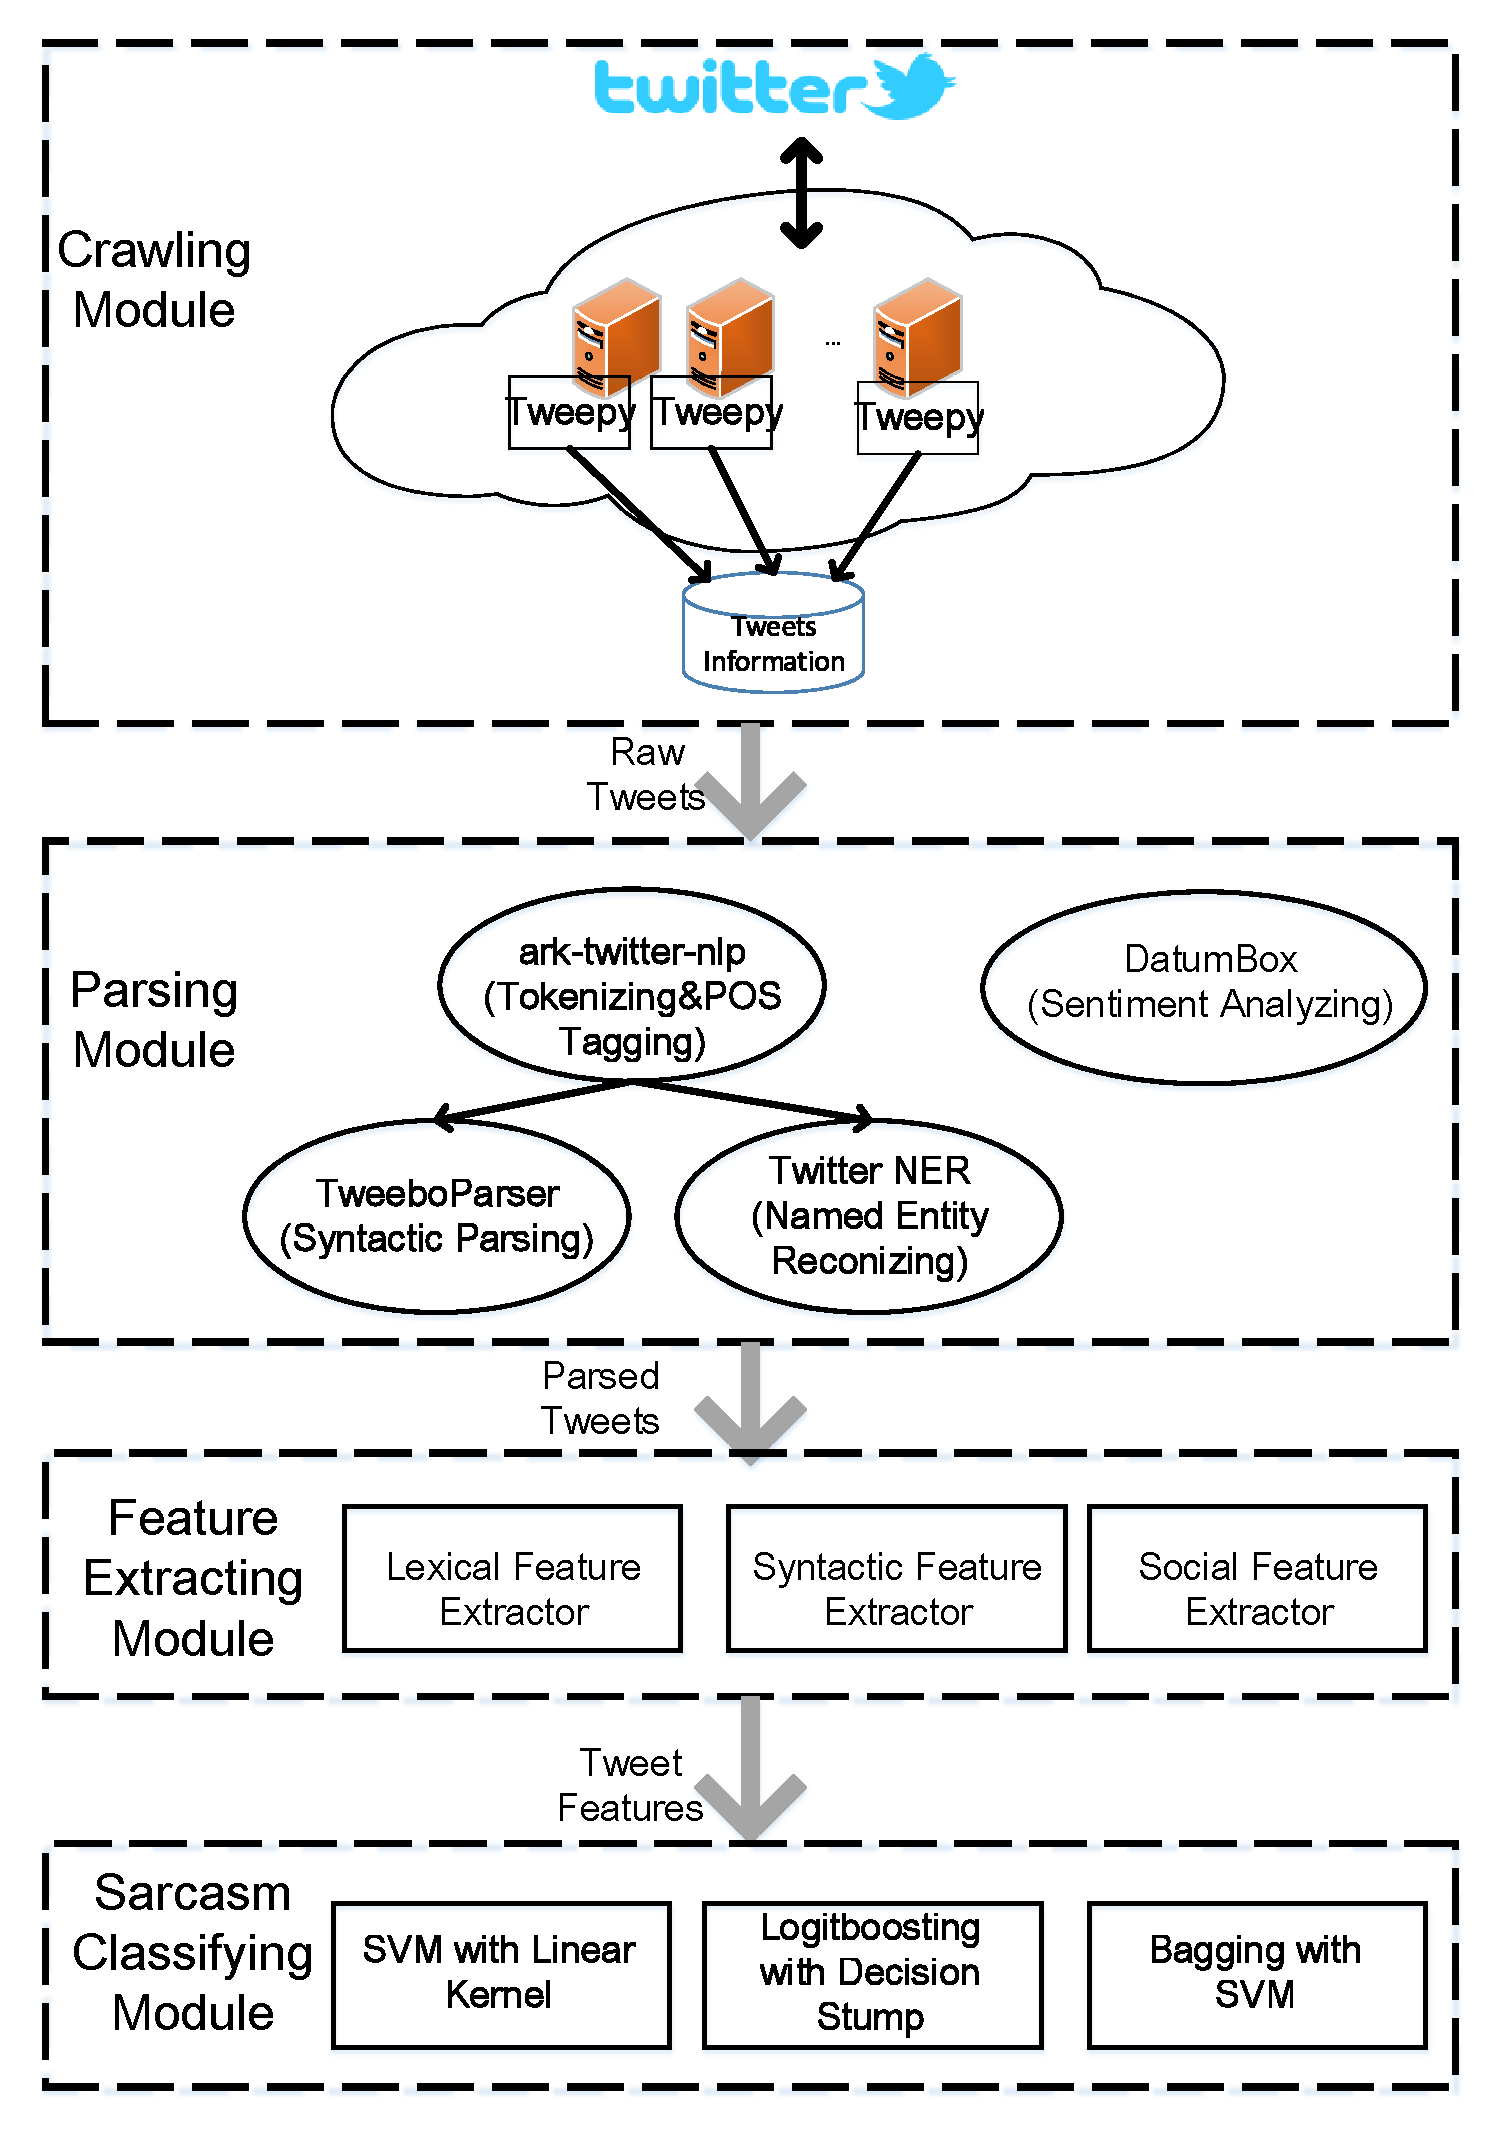
\includegraphics[scale=0.3]{infrastructure.eps}
\caption{The infrastructure of system setup.}
\label{fig:infrastructure}
\end{figure}

\section{Evaluation and Discussion}
\label{sec:evaluation}
This is evaluation.

\begin{figure}[hbt]
\centering
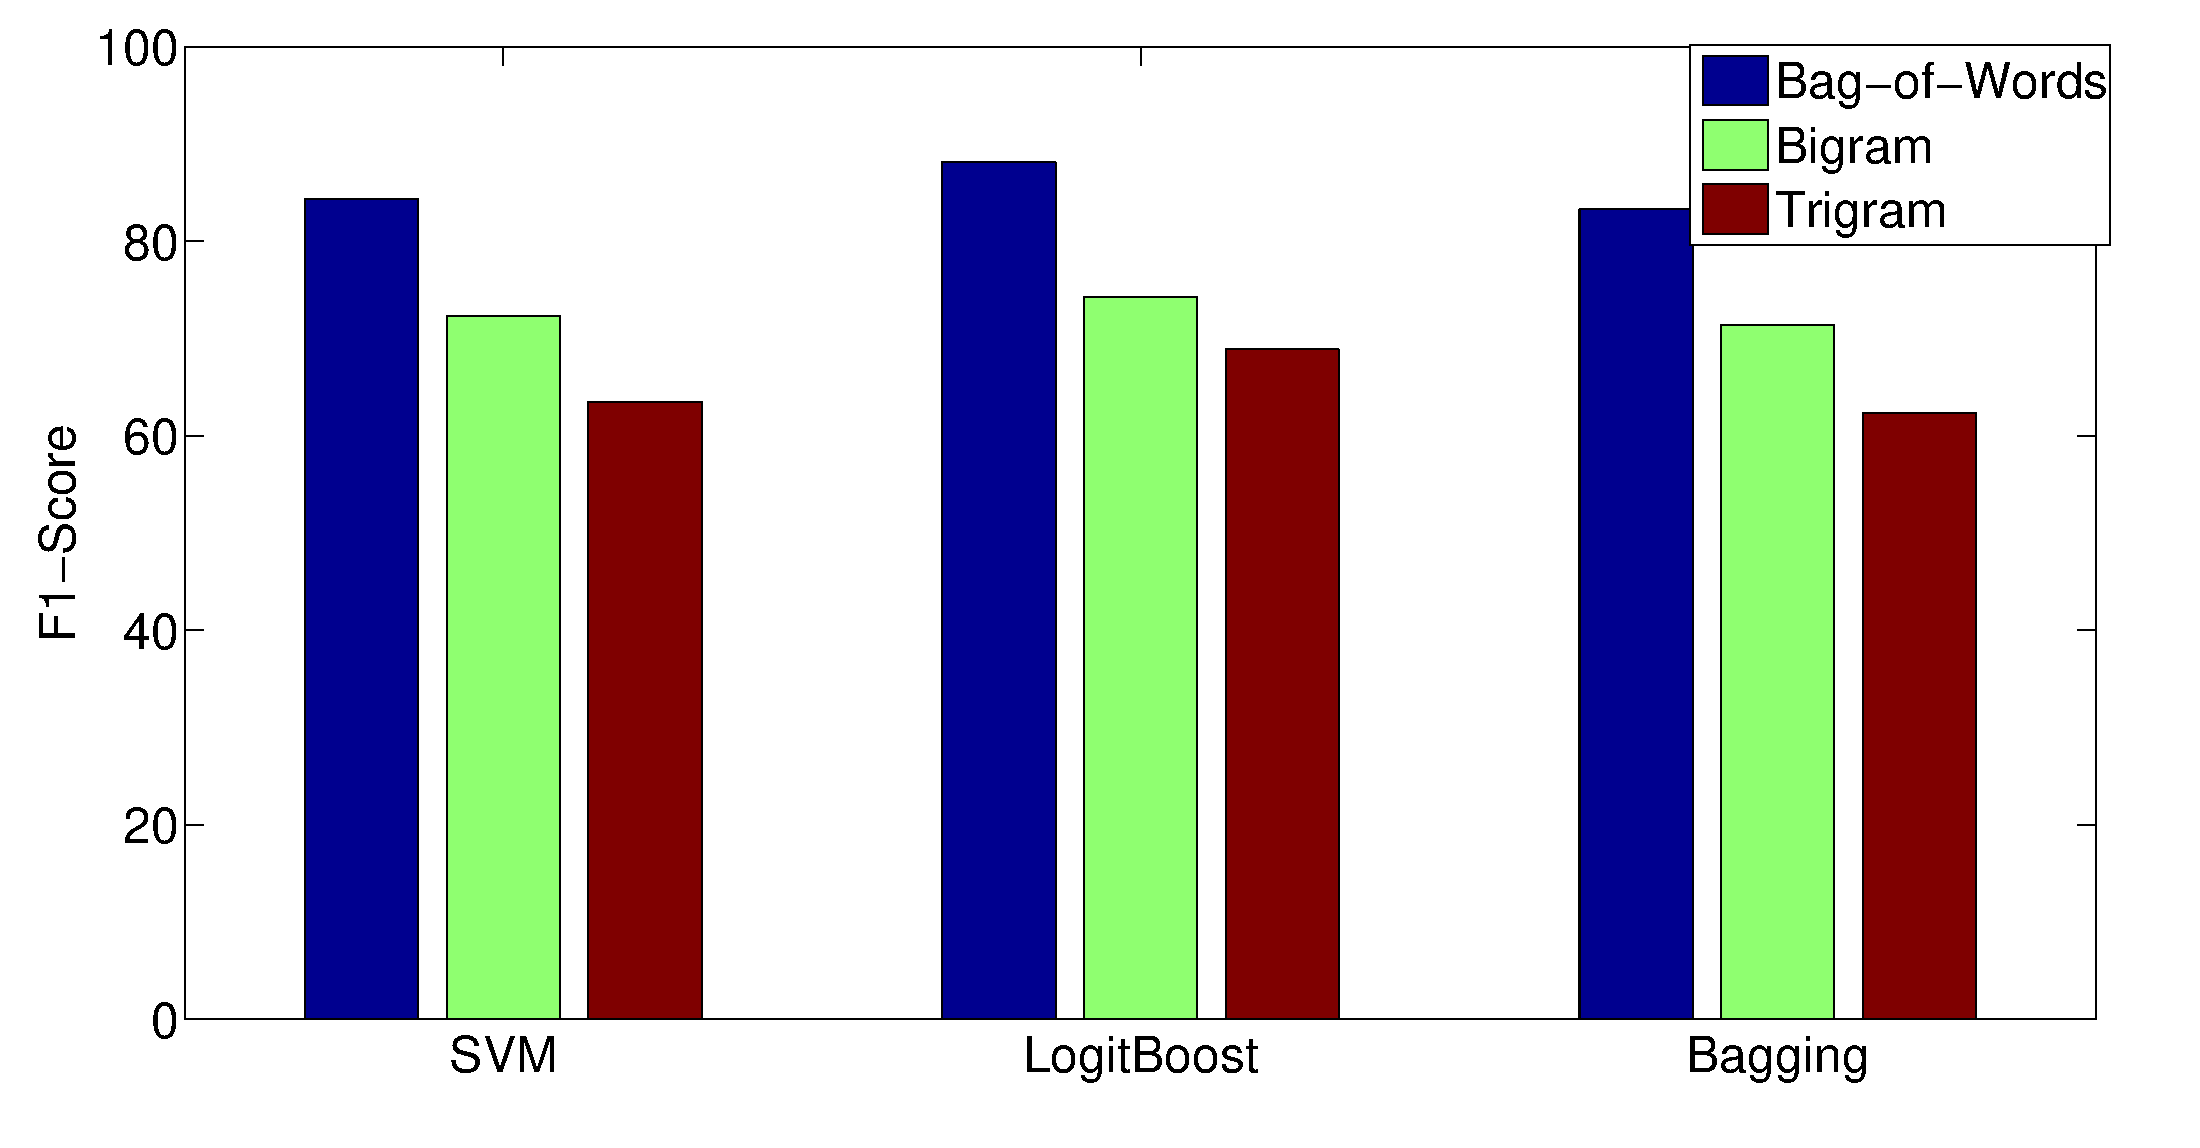
\includegraphics[width=3.4in, height= 2.4 in]{./figs/bow.eps}
\caption{Effect of different language model specific training in different SSD classifiers}
\label{train:fig}
\end{figure}

\begin{figure}[hbt]
\centering
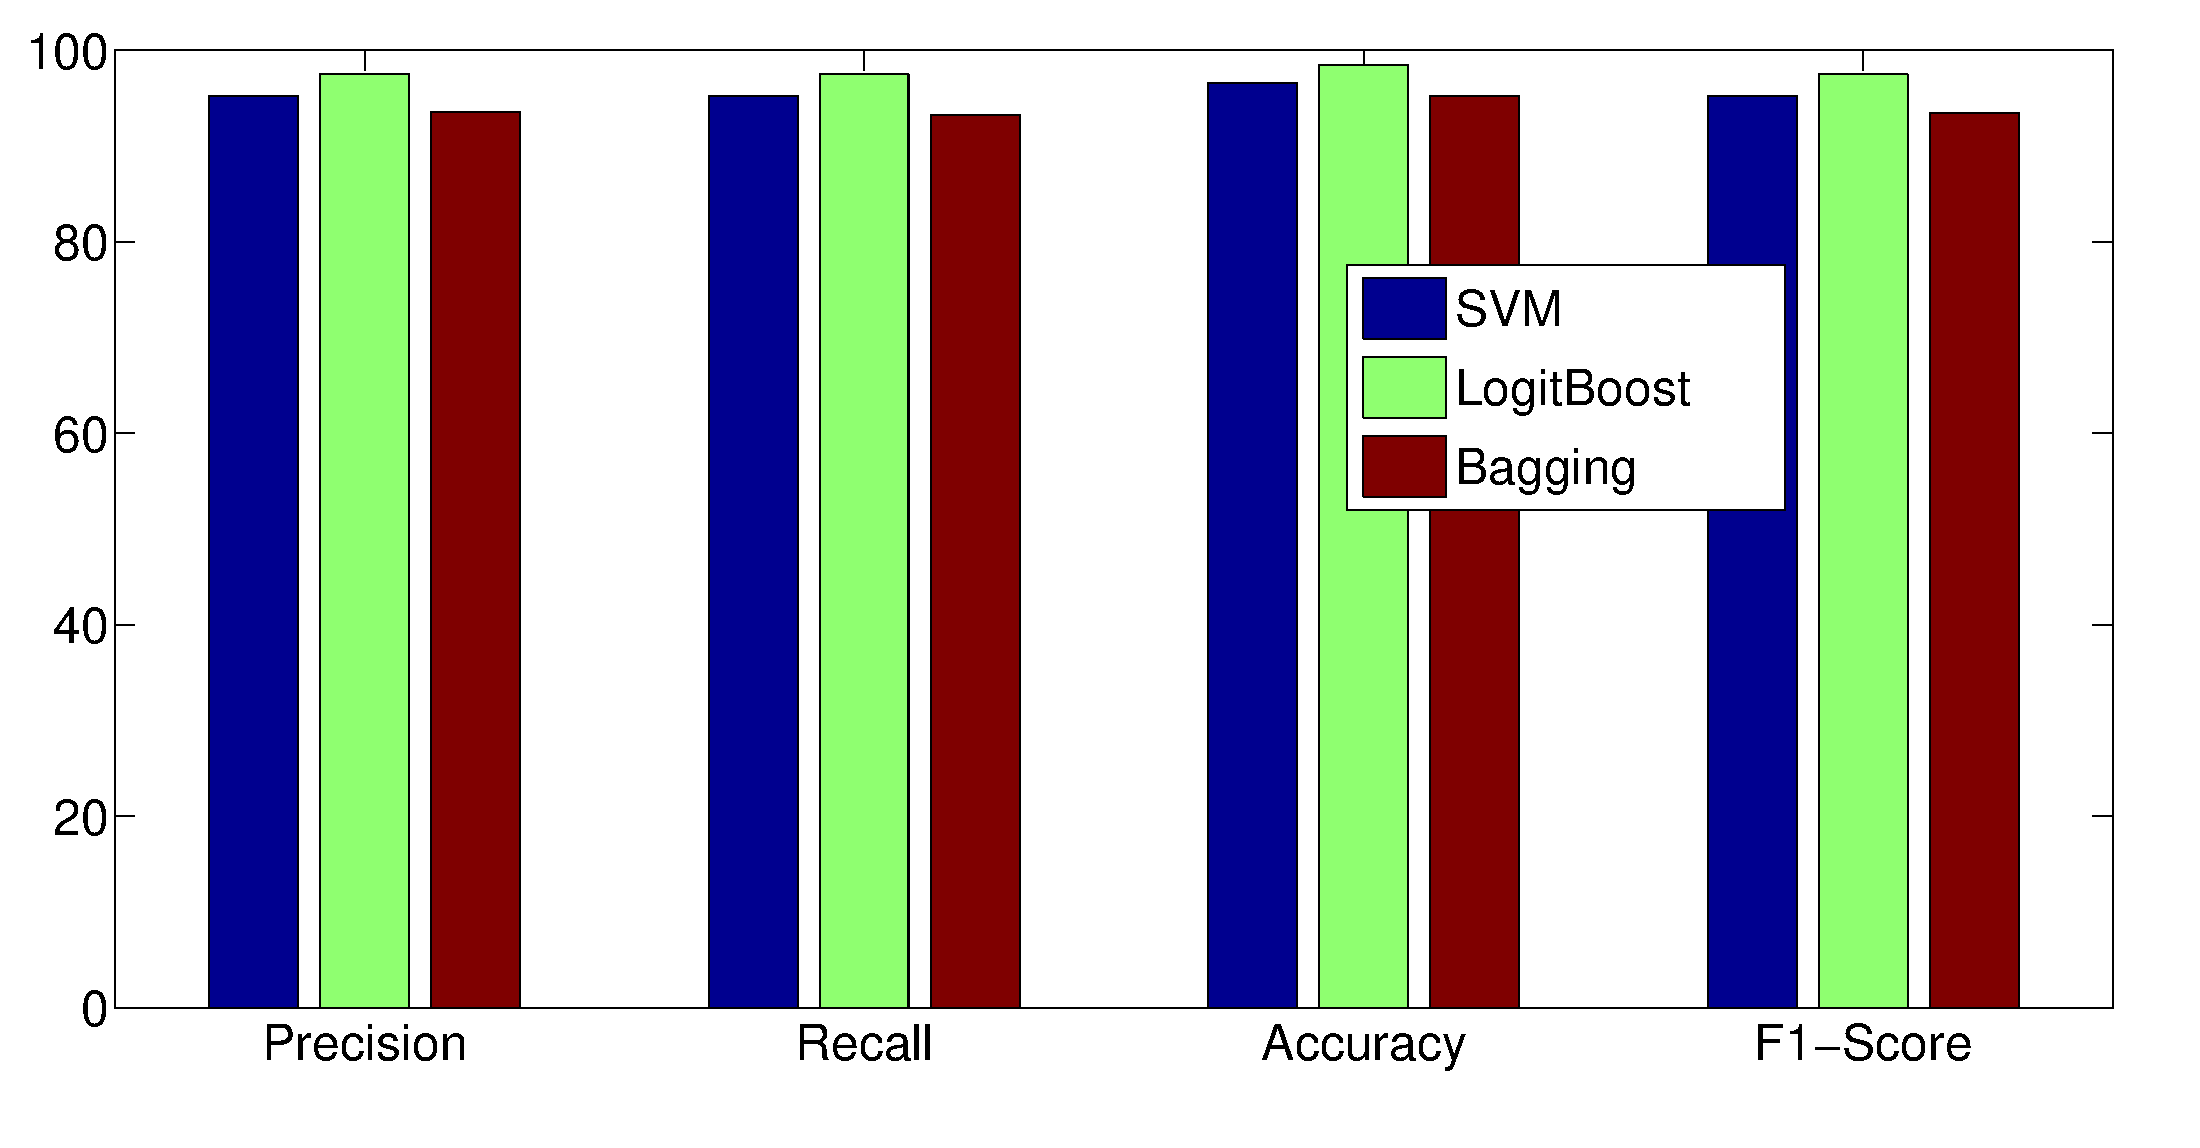
\includegraphics[width=3.4in, height= 2.4 in]{./figs/class.eps}
\caption{Comparison of Precision, Recall, F1-Score and Accuracy of different SSD classifiers}
\label{train:fig}
\end{figure}

\begin{table*}[htb]
%\renewcommand{\arraystretch}{1.9}
  \centering
  {\small
    %\vspace{-0.1in}
  \begin{tabular}{|@{~}l@{~~}|@{~~}l@{~}|@{~~}l@{~}|@{~~}l@{~}|@{~~}l@{~}|@{~~}l@{~}|@{~~}l@{~}|}
\hline
Feature set & Method used & Precision & Recall & Accuracy & F1-Score & AUC \\\hline
Bag-of-Words & SVM with linear kernel & $84.0475$ & $84.6621$ & $83.6177$ & $84.3674$ & $86.5413$ \\\hline
Word Bigram & SVM with linear kernel & $72.0175$ & $72.3411$ & $73.5127$ & $72.3132$ & $77.1137$  \\\hline
Word Trigram & SVM with linear kernel & $63.8823$ & $63.2914$ & $64.7732$ & $63.4913$  & $67.3412$  \\\hline
Only Lexical Feature & SVM with linear kernel & $62.0813$ & $62.2723$ & $65.1184$ & $62.3213$   & $68.9023$ \\\hline
Only Syntactic Feature & SVM with linear kernel & $58.5623$ & $59.4112$ & $61.5234$ & $58.8232$  & $66.6784$ \\\hline
All Features with Social Features & SVM with linear kernel & $\mathbf{95.2358}$ & $\mathbf{95.2218}$ & $\mathbf{96.6023}$ & $\mathbf{95.2123}$   & $\mathbf{97.7812}$ \\\hline
Bag-of-Words & Logitboost\footnote{http://www.cs.waikato.ac.nz/ml/weka/}with Decision Stump & $88.1239$ & $88.1239$ & $90.0324$ & $88.1239$  & $92.2013$  \\\hline
Word Bigram & Logitboost with Decision Stump & $73.3487$ & $74.2375$ & $76.5123$ & $74.2234$   & $79.7613$ \\\hline
Word Trigram & Logitboost with Decision Stump & $68.8812$ & $68.8812$ & $72.1276$ & $68.8812$   & $74.2314$ \\\hline
Only Lexical Feature & Logitboost with Decision Stump & $64.0823$ & $64.0823$ & $67.4098$ & $64.0823$  & $70.2349$  \\\hline
Only Syntactic Feature & Logitboost with Decision Stump & $60.6756$ & $60.6756$ & $63.5454$ & $60.6756$  & $64.0873$ \\\hline
All Features with Social Features & Logitboost with Decision Stump & $\mathbf{97.4568}$ & $\mathbf{97.4568}$ & $\mathbf{98.4176}$ & $\mathbf{97.4568}$ & $\mathbf{98.8876}$ \\\hline
Bag-of-Words & Bagging with SVM \footnote{http://homes.esat.kuleuven.be/~claesenm/ensemblesvm/}& $83.0475$ & $83.5611$ & $84.5177$ & $83.2674$ & $85.3413$ \\\hline
Word Bigram & Bagging with SVM & $71.2713$ & $71.4531$ & $73.3427$ & $71.3412$  & $75.1745$ \\\hline
Word Trigram & Bagging with SVM & $62.8845$ & $62.2914$ & $68.7732$ & $62.3457$ & $70.3456$ \\\hline
Only Lexical Feature & Bagging with SVM  & $58.0823$ & $58.0127$ & $61.2384$ & $58.0432$  & $63.4523$  \\\hline
Only Syntactic Feature & Bagging with SVM  & $53.1256$ & $53.1256$ & $56.8674$ & $53.1256$  & $59.0234$ \\\hline
All Features with Social Features & Bagging with SVM & $\mathbf{93.5812}$ & $\mathbf{93.1846}$ & $\mathbf{95.1456}$ & $\mathbf{93.4054}$  & $\mathbf{97.3216}$ \\\hline
%\vspace{-0.15in}
\end{tabular}
  }
 \vspace{0.05in}
  \caption{Summary of Results for running SVM, Boosting, and Bagging with different feature sets on datasets.}
%\vspace{-0.25in}
  \label{tab:data1}
\end{table*}

\begin{figure}[hbt]
\centering
\includegraphics[width=3.4in, height= 2.4 in]{./figs/compare_systems.eps}
\caption{Comparison of a few competing techniques with SSD}
\label{train:fig}
\end{figure}

\begin{table}[htb]
%\renewcommand{\arraystretch}{1.9}
  \centering
  {\small
    %\vspace{-0.1in}
  \begin{tabular}{|@{~}l@{~~}|@{~~}l@{~}|@{~~}l@{~}|@{~~}l@{~}|@{~~}l@{~}|}
\hline
Technique & Precision & Recall & F1-Score & Accuracy\\\hline
SASI \cite{davidov10} & $74.27$ & $70.67$ & $72.43$ & $78.68$\\\hline
Coling '14 \cite{tomas14} & $91.23$ & $91.23$ & $91.23$ & $95.77$\\\hline
SSD & $97.46$ & $97.46$ & $97.46$ & $98.89$\\\hline
%\vspace{-0.15in}
\end{tabular}
  }
 \vspace{0.05in}
  \caption{Comparing different supervised techniques of Sarcasm Detection in Twitter with SSD}
%\vspace{-0.25in}
  \label{tab:data2}
\end{table}

% \begin{table}[htb]
% %\renewcommand{\arraystretch}{1.9}
%   \centering
%   {\small
%     %\vspace{-0.1in}
%   \begin{tabular}{|@{~}l@{~~}|@{~~}l@{~}|@{~~}l@{~}|@{~~}l@{~}|@{~~}l@{~}|}
% \hline
% Technique & Precision & Recall & F1-Score & Accuracy\\\hline
% SASI (CoNLL 2010) & $50.67$ & $48.27$ & $49.44$ & $52.68$\\\hline
% Coling 2014 & $53.23$ & $53.23$ & $53.23$ & $59.77$\\\hline
% SSD & $65.46$ & $65.46$ & $65.46$ & $68.89$\\\hline
% %\vspace{-0.15in}
% \end{tabular}
%   }
%  \vspace{0.05in}
%   \caption{Comparing different techniques Sarcasm Detection in Twitter in Czech Dataset}
% %\vspace{-0.25in}
%   \label{tab:data2}
% \end{table}
\section{Future Work}
\label{sec:future}
This is Future Work.
%\input{emoapp}
%\input{path_forward}
%\section{Related Work}
\textbf{Image based Facial Expression Detection : }In the past years, the literature on automatic facial expression recognition has grown dramatically by applying advanced techniques of image and video processing. Most studies of automatic facial expression recognition focus on six primary facial expressions or a subset of them, namely happiness, sadness, anger, fear, surprise, and disgust. The expression and recognition of these primary facial expressions were found in Ekman’s extensive studies\cite{ekman} to be universal in different cultures. The studies of computer-assisted recognition of facial expressions started in 1990s. Mase\cite{mase} explored the technique of optical flow for facial expressions recognition. Lanitis et al.\cite{lanitis} applied a flexible shape and appearance model to recognize person identities, genders and facial expressions. Black and Yacoob\cite{black95} used local parameterized models of image motion to track non-rigid facial motion that was fed to a rule-based classifier of facial expressions. Rosenblum et al.\cite{rosenblum} used optical flow and a radial basis function network to
classify expressions. Otsuka and Ohya\cite{otsuka97} used optical flow and a hidden Markov model (HMM) for facial expression
recognition. Tian et al\cite{tian} explored action unit recognition by using multi-state facial component models and a neural-network-based classifier. Cohen et al.\cite{cohen03} introduced the structure of Bayesian network classifiers and a multi-level HMM classifier to automatically segment an arbitrary long sequence to the corresponding facial expressions. For extensive survey of facial expression analysis using images done in the recent years, readers are referred to the overview papers, including \cite{pantic00,pantic03} written by Pantic and Rothkrantz in 2000 and 2003.\\

\textbf{EEG based Expression and Emotion Detection : }Several works have attempted recognition of emotions from EEG signals. In \cite{channel2009}, participants are asked to remember an episode in their life that corresponds to positive/excited and one that corresponds to negative/excited emotions. A third emotional state called calm/neutral is elicited by asking the participants to stay calm and relax. For these three classes, a classification accuracy of 63\% is reported using the short-time Fourier transform for feature extraction and a linear SVM for classification. In \cite{deap}, participants watch a series of music videos selected to elicit emotions. The participants then rate the felt emotions in terms of valence, arousal and like/dislike. In performing a binary classification, accuracies of up to 62\% are attained based on EEG band-power features and a Gaussian Naïve Bayes classifier. Regression results for the same experiment are reported in \cite{soleymani}. In \cite{takahashi}, 5 different emotions (joy, anger, sadness, fear, and relaxation) are elicited by using video stimuli in 12 participants. Using a one-vs-all SVM classifier, a classification rate of 41.7\% is reported. Besides these works, much research has been done in psychology into ERP analysis and correlations with emotion (e.g. \cite{olof,cuthbert}). These works show clear associations between ERP activity and valence/arousal. However, they mostly have in common that they work with time-locked stimuli (such as pictures), and average the ERP signal over several trials to increase the signal-to-noise ratio. However, all these works do not concentrate upon the facial expression detection cum emotion recognition which we attempt to address.
\section{Conclusion}
\label{sec:conclusion}
In this project, we have collected and consolidated a reasonable amount of sarcastic tweets for the evaluation purpose. We have also shown that if we include different socio-contextual feature which basically represents world knowledge, we can achieve better accuracy in sarcasm prediction. There is also inherent variety of sarcastic tweets which needs to be tackled differently. Using different supervised machine learning techniques, with these diverse set of features, we have achieved better F1-score compared to different state-of-the-art techniques.

\bibliographystyle{abbrv}
{\footnotesize\bibliography{final_report}}

\end{document}
